\subsection{Task Coalescing}

\begin{algorithm}
	\caption{Coalescing}
	\label{algo:genCoalescing}
	\scriptsize
	%\small
	\begin{algorithmic}[1]
        \State $H_\text{p} \gets H_\text{c}$
        \State $H_\text{p} \gets 0$ 
        \State $H_\text{B} \leftarrow $ \Call{$f_\text{reboot}$}{B, $H_\text{p}$}

        \While{$\texttt{true}$}
	        \State $ B_\text{c} \gets B$
	        \While{$ B_\text{c} > 0$}
		        \State \Call{execute\_task}{$T_\texttt{i}$}
		        % \State $W$ \gets \Call{f_\text{weight}}{$T_\texttt{i}$}
		        \State $B_\text{c} \gets B_\text{c} - W$
				\State $H_\text{c} \gets H_\text{c} + W$
	        \EndWhile
	        % \State $B$ \gets \Call{f\_compl}{$\texttt{B},\texttt{H_\text{c}},\texttt{H_\text{p}}$}
	        \State \Call{commit\_to\_fram}{}
        \EndWhile
	\end{algorithmic}
\end{algorithm}

%% Coalescing motivation
Finding an optimal task size, given random energy conditions is an open question. Obviously, a static approach does not have the potential to answer it. Therefore, \sys champions runtime-based methods to approximate the ideal task size under random energy shots arrival. Furthermore, \sys advocates making intermittently powered software energy-aware is the key for \emph{efficient code execution and probability}. 
%However, given the extremely limited recourses any optimization technique must adhere to the principle of simplicity, otherwise it introduces a non-tolerable overhead. 

% %% address the challenge and define the optimal task
\sys advances its execution in a state-less (or virtual) manner, and then it frequently saves its forward progress. The longer \sys virtually progresses, the less committing (saving data to non-volatile memory) overhead it introduces. However, long state-less execution results in a considerable re-execution penalty---all the tasks that have been virtually executed must be re-executed after a power interrupt. As such, an optimal task is a task that occupies with a single commit an entire power cycle, which is therefore necessarily of a varying length.  

% %% How does Coala approximates an ideal task
\sys adapts its virtual execution by mean of \emph{coalescing} static tasks, when energy permits, to optimally execute an intermittently powered program. It devises a number of coalescing algorithms, and states that a good coalescing strategy must moderate the risk of wasted work (re-execution penalty) and capitalize on benefits of deferred commits. To describe the proposed strategies we will use the following parameters: \\
(i) \textit{target budget B}: total number of units to coalesce; (ii) \textit{current budget $B_\text{c}$}: remaining number of tasks to be coalesced before committing to non-volatile memory; (iii) \textit{history H}: total number of tasks executed in the current discharge cycle, initialized to the number of executed tasks in the last power cycle. 

The general structure of the proposed coalescing strategies is summaries in algorithm~\ref{algo:genCoalescing}, where where $H_\text{p}$, $H_\text{c}$, $B$ and $B_\text{c}$ represent past history, current history, target budget and current budget, respectively. $T_\text{i}$ is the i-th task being executed and $W$ is its weight.
A coalescing strategy and its performance are defined by the functions: \\
(i) \emph{$f_\text{reboot}$}: which updates the target budget after a reboot; (ii) \emph{$f_\text{weight}$}: which returns the weight of the task just executed and its unit; (iii) \emph{$f_\text{compl}$}: which updates the target budget after a successful completion of a dynamic coalesced task. The following sections detail the different strategies \sys proposes and the needs that originated from one strategy leading to the conception of another one.

\subsubsection{SC: Slow Coalescing}
\label{subsec:slowCoalescing}

\begin{figure}
	\centering
	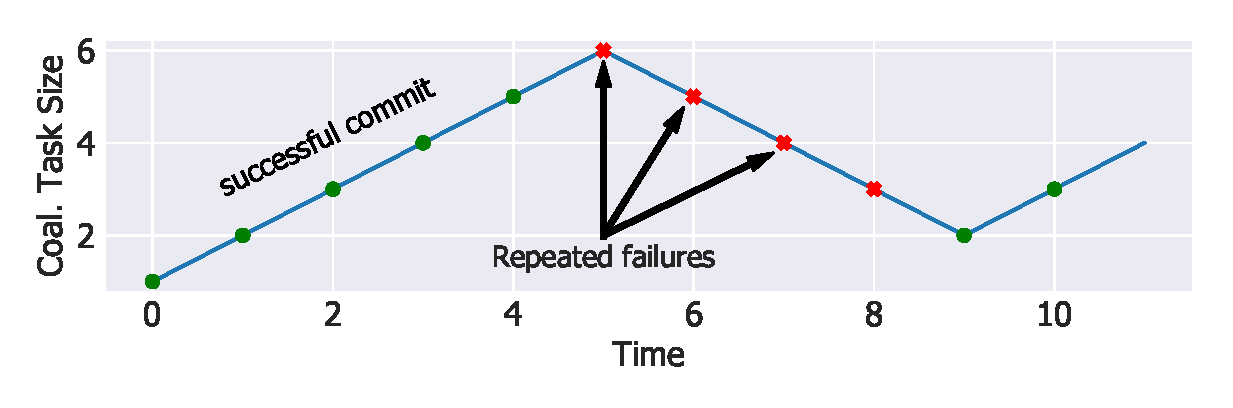
\includegraphics[width=\columnwidth]{figures/slowCoal}%coalescing_timeline
	\caption{The Slow coalescing algorithm \emph{linearly} updates its coalescing target}
	\label{fig:slowCoal}
\end{figure}

The need for \emph{adaptiveness}, that is coalescing static tasks, can be fulfilled by a naive strategy, having the target budget $B$ to increase by $x$ static tasks after a successful completion of a coalesced task, and to decrease by the same number of tasks upon a reboot. In this case: $f_\text{reboot} = B - x$; $f_\text{weight} =  1$; $f_\text{compl} = B + x$; \\
Due to the linear behavior of the target adaptation, this algorithm is slow in reacting to the changes in energy conditions; the energy required by a coalesced task or the available energy. In particular, this algorithm can experience a large number of \emph{repeated power} failures without forward progress.

\subsubsection{HC: History-aware Coalescing}
\label{subsec:hCCoalescing}

\begin{figure}
	\centering
	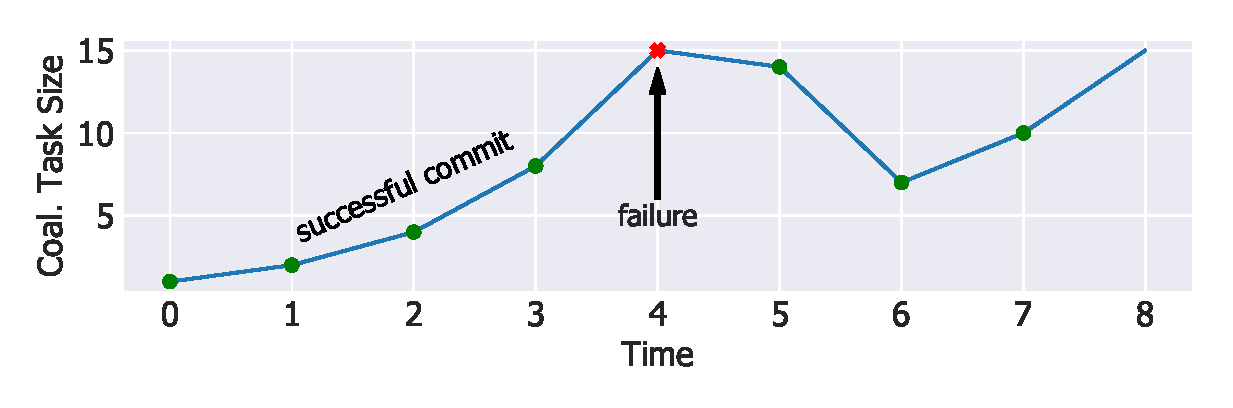
\includegraphics[width=\columnwidth]{figures/HCCoal}%coalescing_timeline
	\caption{The History-aware coalescing algorithm  updates its coalescing target}
	\label{fig:HCCoal}
\end{figure}

The History-aware algorithm uses its recent execution history as metric to estimate the optimal coalesce task size. Relying on the history of execution enables this algorithm to react very quickly to discharge rates variation. 
